\documentclass{article}
\usepackage[T1]{fontenc}
\usepackage{fancyhdr}
\usepackage{extramarks}
\usepackage{amsmath}
\usepackage{amsthm}
\usepackage{amsfonts}
\usepackage{dsfont}
\usepackage{tikz}
\usepackage[plain]{algorithm}
\usepackage{algpseudocode}
\usepackage{graphicx}
\usepackage{listings}
\usepackage{enumitem}

\graphicspath{ {./../img} }

\usetikzlibrary{automata,positioning}

%
% Basic Document Settings
%

\topmargin=-0.45in
\evensidemargin=0in
\oddsidemargin=0in
\textwidth=6.5in
\textheight=9.0in
\headsep=0.25in

\linespread{1.1}

\pagestyle{fancy}
\lhead{\hmwkAuthorName}
\chead{\hmwkTitle}
\rhead{\hmwkClass}
\lfoot{\lastxmark}
\cfoot{\thepage}

\renewcommand\headrulewidth{0.4pt}
\renewcommand\footrulewidth{0.4pt}

\setlength\parindent{0pt}
\setlength{\parskip}{5pt}

%
% Homework Details
%   - Title
%   - Due date
%   - Class
%   - Section/Time
%   - Instructor
%   - Author
%

\newcommand{\hmwkTitle}{Quiz\ \#5}
\newcommand{\hmwkDueDate}{December 8, 2023}
\newcommand{\hmwkClass}{ECE 271A}
\newcommand{\hmwkClassInstructor}{Professor Vasconcelos}
\newcommand{\hmwkAuthorName}{\textbf{Ray Tsai}}
\newcommand{\hmwkPID}{A16848188}

%
% Title Page
%

\title{
    \vspace{2in}
    \textmd{\textbf{\hmwkClass:\ \hmwkTitle}}\\
    \normalsize\vspace{0.1in}\small{Due\ on\ \hmwkDueDate\ at 11:59pm}\\
    \vspace{0.1in}\large{\textit{\hmwkClassInstructor}} \\
    \vspace{3in}
}

\author{
  \hmwkAuthorName \\
  \vspace{0.1in}\small\hmwkPID
}
\date{}

%
% Various Helper Commands
%

% Useful for algorithms
\newcommand{\alg}[1]{\textsc{\bfseries \footnotesize #1}}

% For derivatives
\newcommand{\deriv}[1]{\frac{\mathrm{d}}{\mathrm{d}x} (#1)}

% For partial derivatives
\newcommand{\pderiv}[2]{\frac{\partial}{\partial #1} (#2)}

% Integral dx
\newcommand{\dx}{\mathrm{d}x}

% Probability commands: Expectation, Variance, Covariance, Bias
\newcommand{\Var}{\mathrm{Var}}
\newcommand{\Cov}{\mathrm{Cov}}
\newcommand{\Bias}{\mathrm{Bias}}
\newcommand*{\Z}{\mathbb{Z}}
\newcommand*{\Q}{\mathbb{Q}}
\newcommand*{\R}{\mathbb{R}}
\newcommand*{\C}{\mathbb{C}}
\newcommand*{\N}{\mathbb{N}}
\newcommand*{\prob}{\mathds{P}}
\newcommand*{\E}{\mathds{E}}
\newcommand*{\G}{\mathcal{G}}
\newcommand*{\D}{\mathcal{D}}

\begin{document}

\maketitle

\pagebreak

\section*{Part A}

For each class, learn 5 mixtures of $C = 8$ components, using a random initialization (recall that the
mixture weights must add up to one). Plot the probability of error vs. dimension for each of the 25
classifiers obtained with all possible mixture pairs. Comment the dependence of the probability of error
on the initialization.
\\

\textbf{\large Solution}
\\

Note that the $Q$ function in the $E$-step is
\begin{align*}
    Q(\mu, \Sigma, \pi, ; \Psi^{(n)}) = \sum_{ij} h_{ij} \log[\G(x_i, \mu_j, \Sigma_j)\pi_j],
\end{align*}
where,
\[
    h_{ij} = P_{Z|X}(e_j | x_i ; \Psi^{(n)}) = \frac{\G(x_i, \mu_j^{(n)}, \Sigma_j^{(n)})\pi_j^{(n)}}{\sum_{k = 1}^C \G(x_i, \mu_k^{(n)}, \Sigma_k^{(n)})\pi_k^{(n)}}.
\]
Hence, the updated parameters in the $M$-step are
\[
    \mu_j^{(n + 1)} = \frac{\sum_i h_{ij}x_i}{\sum_i h_{ij}}, \quad \pi_j^{(n + 1)} = \frac{1}{n}\sum_i h_{ij}, \quad \Sigma_j^{(n + 1)} = \frac{\sum_i h_{ij} (x_i - \mu_j^{(n + 1)})(x_i - \mu_j^{(n + 1)})^T}{\sum_i h_{ij}}.
\]
For initialization, we simply take random vectors of some uniform distributions for each parameter.
The following are the performance of the 25 ramdomly initialized mixure models:
\begin{center}
    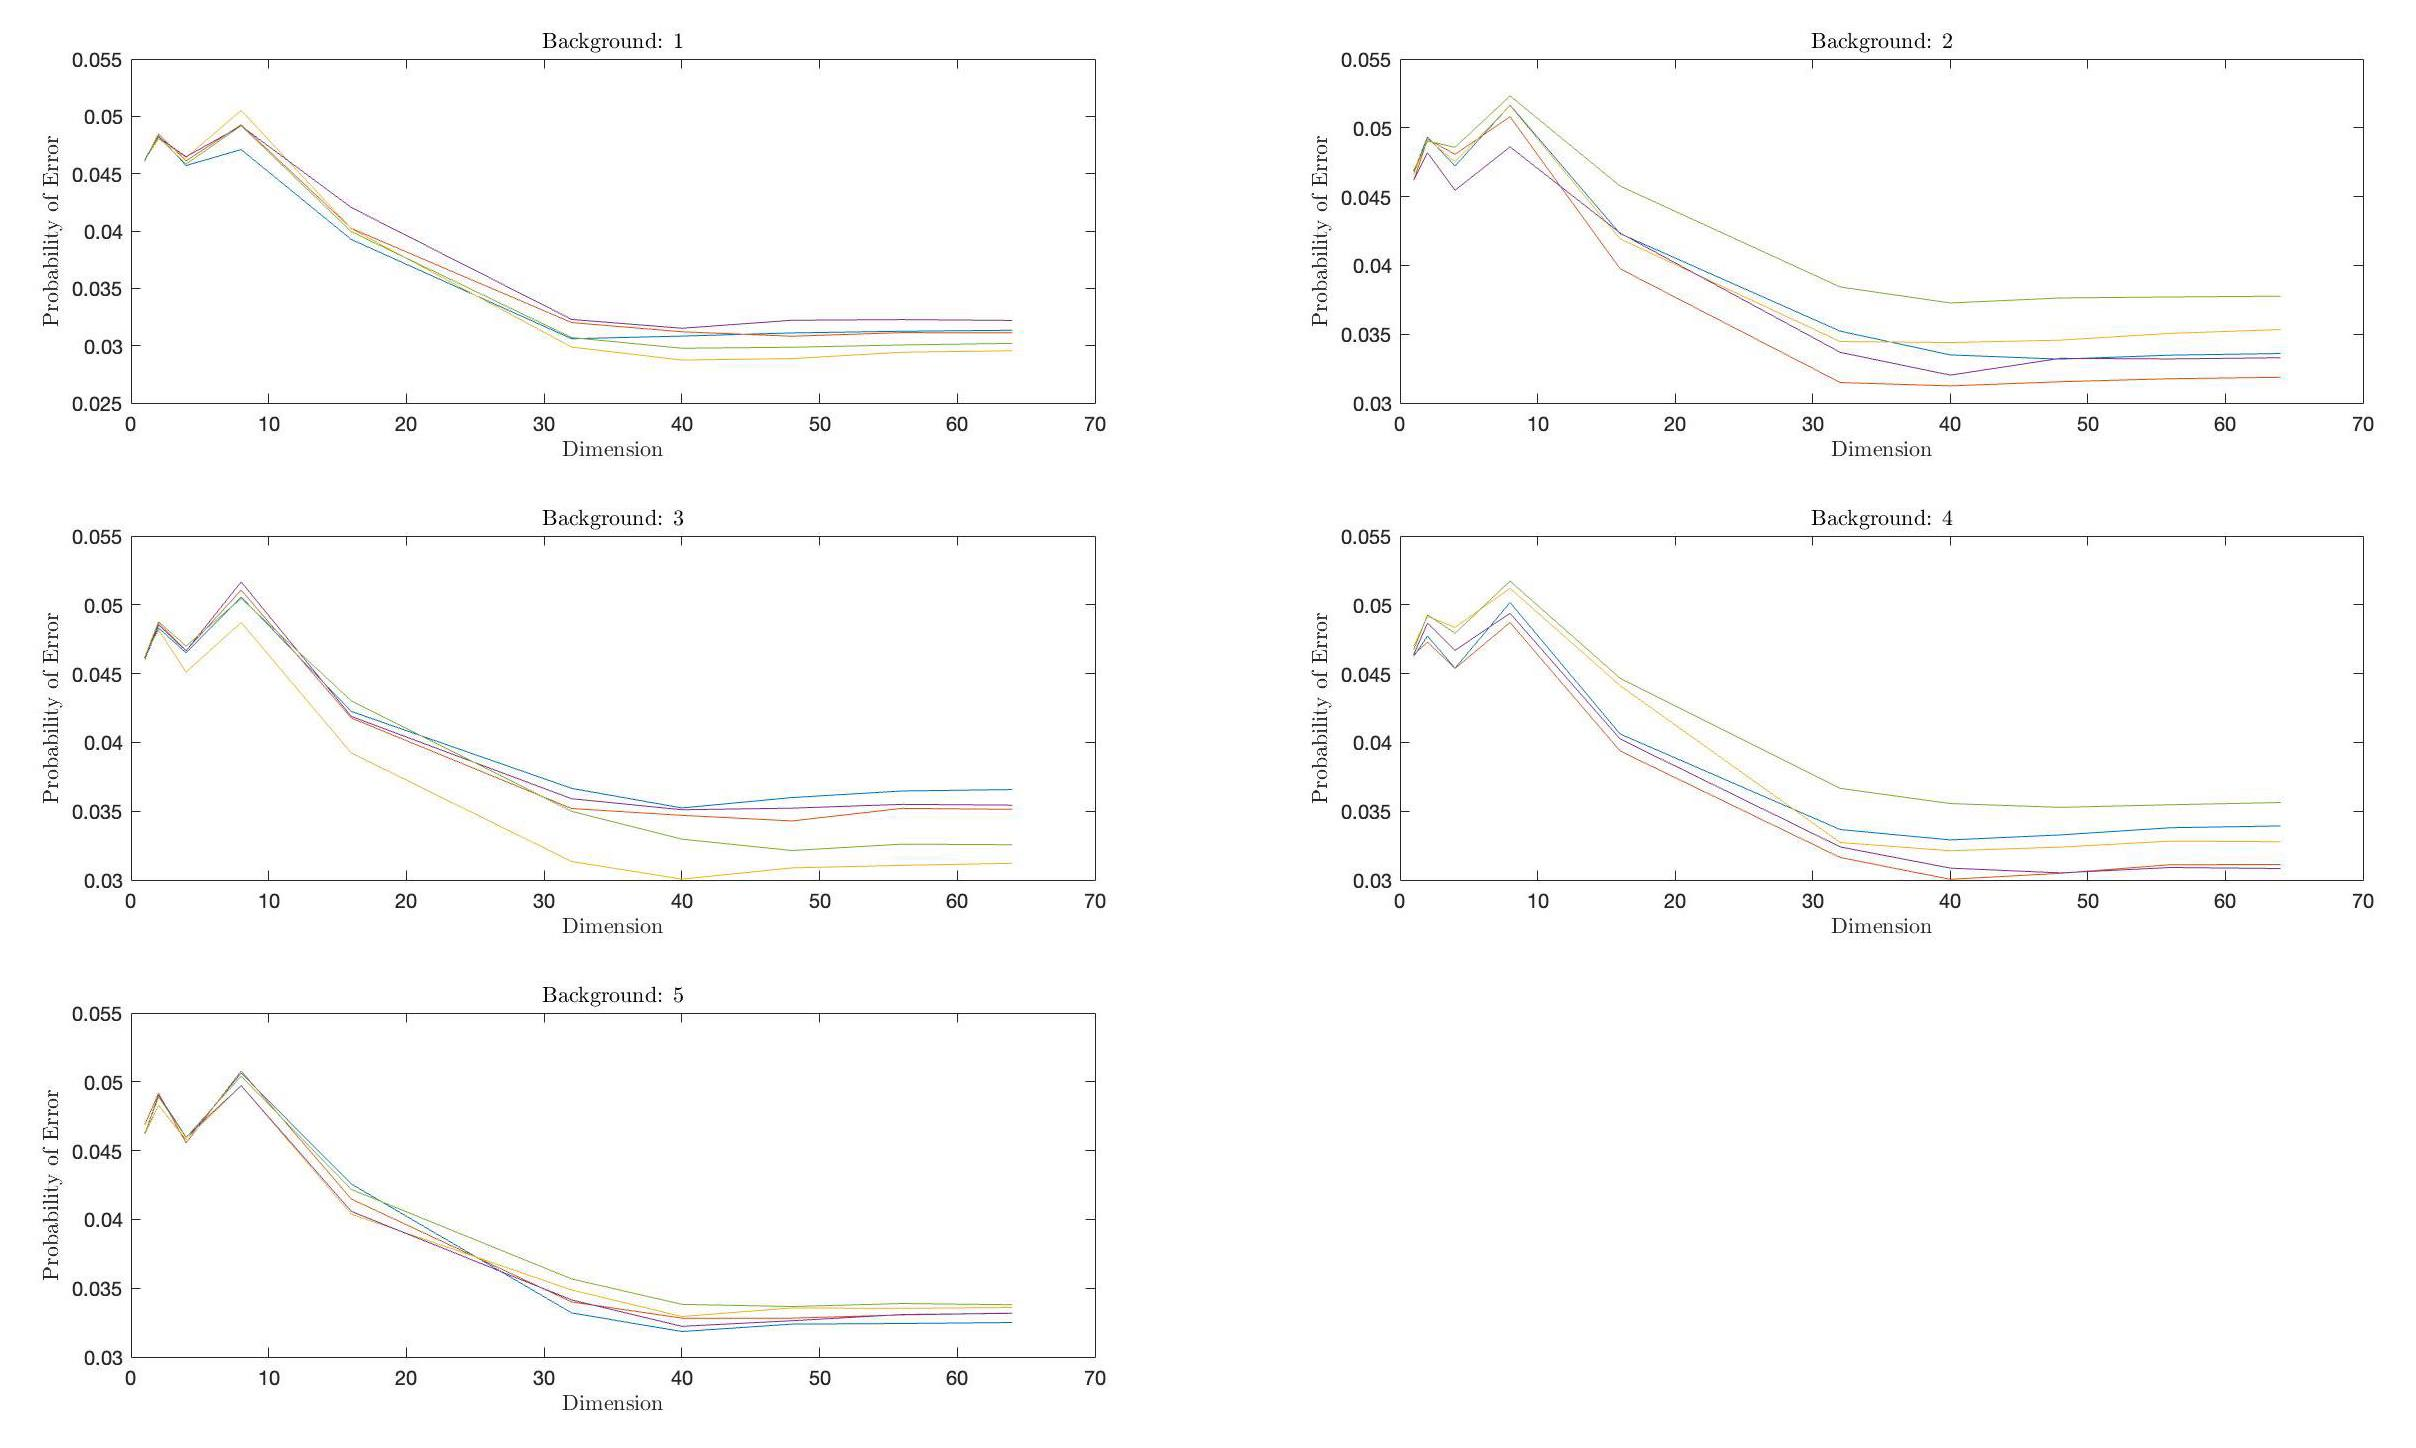
\includegraphics[width=0.99\textwidth]{partA}
\end{center}
As shown in the above figures, the plots all show a similar overall trend, where the probability of error decreases as the dimension increases.
However, the probability of errors accross each plot slightly differs, which is especially prominent in higher dimensions.
This implies that the quality of our initial parameters affects the local maximum that the EM-algorithm converges to.
\\

\section*{Part B}

For each class, learn mixtures with $C \in \{1, 2, 4, 8, 16, 32\}$. 
Plot the probability of error vs. dimension for each number of mixture components. 
What is the effect of the number of mixture components on the probability of error?
\\

\textbf{\large Solution}
\\

\begin{center}
    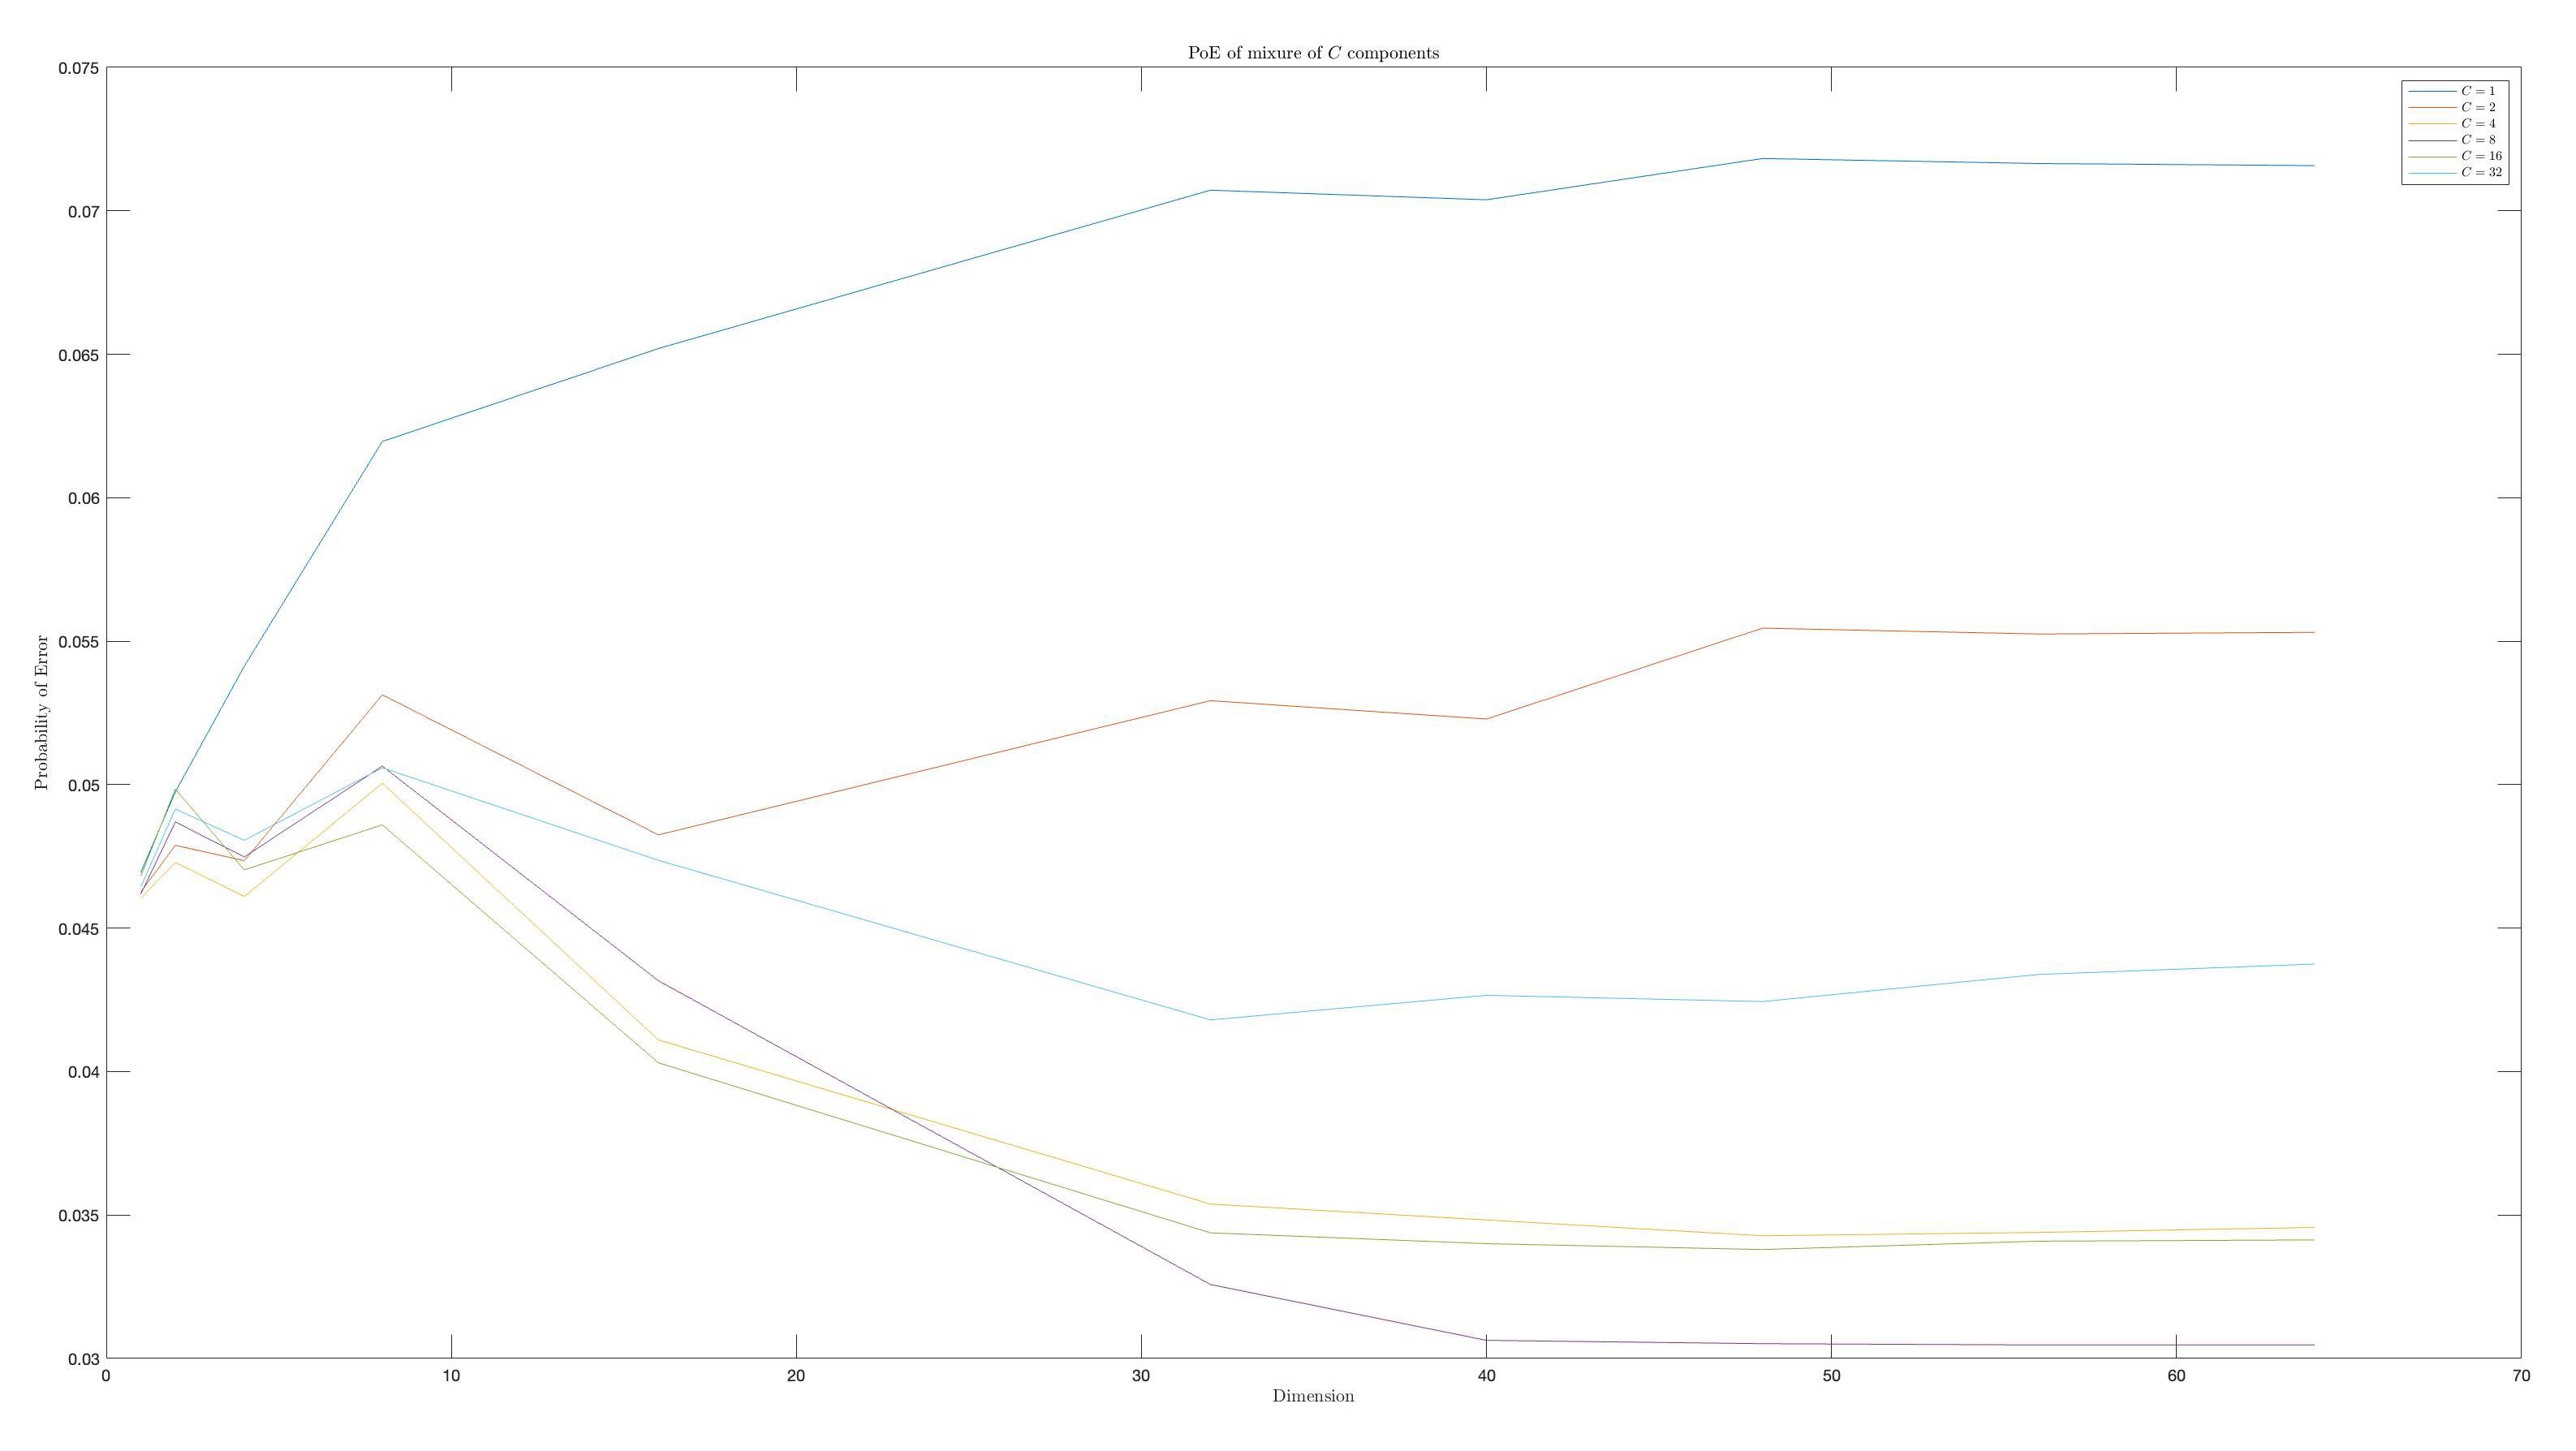
\includegraphics[width=\textwidth]{partB}
\end{center}
From the above figure, we can tell that the increase of number of components does not necessarily increase the performance.
Increasing the number of components of a smaller number, e.g. $C = 1, 2$, does exhibit a significant performance improvement.
However, if the number of components is already large enough, e.g. $C = 8, 16$, increasing the number of components does not necessarily enhance the performance.
This may be due to the difference in initialization, but the extent that it can affect the performace is limited if our initialization method is of a decent quality, as shown in part A.
Therefore, increasing the number of components in the mixure model can only improve the performance to a certain extent, and the optimal number of components might not be the largest one.

\pagebreak

\section*{MATLAB Code}

\subsection*{partA.m}

\begin{lstlisting}[language=Matlab]
load('../dataset/TrainingSamplesDCT_8.mat');
zigzag = load('../dataset/Zig-Zag Pattern.txt');
cheetah = imread('../dataset/cheetah.bmp');
cheetah_mask = imread('../dataset/cheetah_mask.bmp');
target = im2double(cheetah);
mask = im2double(cheetah_mask);

training_BG = TrainsampleDCT_BG;
training_FG = TrainsampleDCT_FG;

[row_BG, col_BG] = size(training_BG);
[row_FG, col_FG] = size(training_FG);
[row_TG, col_TG] = size(target);

zigzag = zigzag + 1;

epoch = 100;

prior_BG = row_BG / (row_BG + row_FG);
prior_FG = row_FG / (row_BG + row_FG);

% pick cheetah if (p(x | grass) / p(x | cheetah)) < threshold
threshold = prior_FG / prior_BG;

mean_FG = sum(training_FG, 1) / row_FG;
mean_BG = sum(training_BG, 1) / row_BG;

dimensions = [1 2 4 8 16 32 40 48 56 64];

C = 8;

error_rates = zeros(5, 5, 10);

for b=1:5

pi_BG = rand(1, C) + 1;
pi_BG = pi_BG / sum(pi_BG);

mu_BG = rand(64, C);
for c=1:C
    mu_BG(:, c) = mu_BG(:, c) + mean_BG';
end

sigma_BG = 1 + rand(64, C);

for itr=1:epoch
    h_BG = zeros(row_BG, C);
    for i=1:row_BG
        for j=1:C
            h_BG(i, j) = mvn(training_BG(i, :), mu_BG(:, j)', ...
                diag(sigma_BG(:, j)')) * pi_BG(j);
        end
        h_BG(i, :) = h_BG(i, :) ./ sum(h_BG(i, :));
    end

    for j=1:C
        pi_BG(j) = sum(h_BG(:, j)) / row_BG;
        temp_mu = zeros(64, 1);
        for i=1:row_BG
            temp_mu = temp_mu + h_BG(i, j) * training_BG(i, :)';
        end
        
        mu_BG(:, j) = temp_mu / sum(h_BG(:, j));
        temp_sigma = zeros(64, 1);
        for i=1:row_BG
            temp_sigma = temp_sigma + h_BG(i, j) * ((training_BG(i, :)' - mu_BG(:, j)).^2);
        end
        sigma_BG(:, j) = temp_sigma / sum(h_BG(:, j));
        sigma_BG(sigma_BG < 0.0001) = 0.0001;
    end
end

disp("Finished EM for BG " + b);

for f=1:5

pi_FG = rand(1, C) + 1;
pi_FG = pi_FG / sum(pi_FG);

mu_FG = rand(64, C);
for c=1:C
    mu_FG(:, c) = mu_FG(:, c) + mean_FG';
end

sigma_FG = 1 + rand(64, C);

for itr=1:epoch
    h_FG = zeros(row_FG, C);
    for i=1:row_FG
        for j=1:C
            h_FG(i, j) = mvn(training_FG(i, :), mu_FG(:, j)', ...
                diag(sigma_FG(:, j)')) * pi_FG(j);
        end
        h_FG(i, :) = h_FG(i, :) ./ sum(h_FG(i, :));
    end

    for j=1:C
        pi_FG(j) = sum(h_FG(:, j)) / row_FG;
        temp_mu = zeros(64, 1);
        for i=1:row_FG
            temp_mu = temp_mu + h_FG(i, j) * training_FG(i, :)';
        end
        
        mu_FG(:, j) = temp_mu / sum(h_FG(:, j));
        temp_sigma = zeros(64, 1);
        for i=1:row_FG
            temp_sigma = temp_sigma + h_FG(i, j) * ((training_FG(i, :)' - mu_FG(:, j)).^2);
        end
        sigma_FG(:, j) = temp_sigma / sum(h_FG(:, j));
        sigma_FG(sigma_FG < 0.0001) = 0.0001;
    end
end

disp("Finished EM for FG " + f);

count = 0;

for d=dimensions
count = count + 1;

sq_sigma_BG = zeros(d, d, C);
for i = 1:C
    sq_sigma_BG(:, :, i) = diag(sigma_BG(1:d, i));
end

sq_sigma_FG = zeros(d, d, C);
for i = 1:C
    sq_sigma_FG(:, :, i) = diag(sigma_FG(1:d, i));
end

gm_BG = gmdistribution(mu_BG(1:d, :)', sq_sigma_BG, pi_BG);
gm_FG = gmdistribution(mu_FG(1:d, :)', sq_sigma_FG, pi_FG);

A = zeros(row_TG, col_TG);

for r = 5:row_TG-3
    for c = 5:col_TG-3
        block = target(r - 4:r + 3, c - 4:c + 3);
        dctBlock = dct2(block);
        X = zeros(1, 64);
        for i = 1:8
            for j = 1:8
                X(zigzag(i, j)) = dctBlock(i, j);
            end
        end
        A(r, c) = int8(pdf(gm_BG, X(1:d)) / pdf(gm_FG, X(1:d)) <= threshold);
    end
end

error = 0;
for r = 1:row_TG
    for c = 1:col_TG
        if (A(r, c) ~= mask(r, c))
            error = error + 1;
        end
    end
end

error_rate = error / (row_TG * col_TG);

disp("Finished inference for BG " + b + ", FG " + f + ", dim " + d + ", error rate is " + error_rate);

error_rates(b, f, count) = error_rate;

end
end
end

figure;

for b=1:5
    subplot(3, 2, b);
    for f=1:5
        plot(dimensions, squeeze(error_rates(b, f, :)));
        hold on;
    end

    title("Background: " + b, 'Interpreter', 'latex');
    
    xlabel("Dimension", 'Interpreter', 'latex');
    ylabel("Probability of Error", 'Interpreter', 'latex');
end
\end{lstlisting}

\pagebreak

\subsection*{partB.m}

\begin{lstlisting}
load('../dataset/TrainingSamplesDCT_8.mat');
zigzag = load('../dataset/Zig-Zag Pattern.txt');
cheetah = imread('../dataset/cheetah.bmp');
cheetah_mask = imread('../dataset/cheetah_mask.bmp');
target = im2double(cheetah);
mask = im2double(cheetah_mask);

training_BG = TrainsampleDCT_BG;
training_FG = TrainsampleDCT_FG;

[row_BG, col_BG] = size(training_BG);
[row_FG, col_FG] = size(training_FG);
[row_TG, col_TG] = size(target);

zigzag = zigzag + 1;

epoch = 100;

prior_BG = row_BG / (row_BG + row_FG);
prior_FG = row_FG / (row_BG + row_FG);

% pick cheetah if (p(x | grass) / p(x | cheetah)) < threshold
threshold = prior_FG / prior_BG;

mean_FG = sum(training_FG, 1) / row_FG;
mean_BG = sum(training_BG, 1) / row_BG;

dimensions = [1 2 4 8 16 32 40 48 56 64];
components = [1 2 4 8 16 32];

error_rates = zeros(6, 10);

for C=components

pi_BG = rand(1, C) + 1;
pi_BG = pi_BG / sum(pi_BG);

mu_BG = rand(64, C);
for c=1:C
    mu_BG(:, c) = mu_BG(:, c) + mean_BG';
end

sigma_BG = 1 + rand(64, C);

for itr=1:epoch
    h_BG = zeros(row_BG, C);
    for i=1:row_BG
        for j=1:C
            h_BG(i, j) = mvn(training_BG(i, :), mu_BG(:, j)', ...
                diag(sigma_BG(:, j)')) * pi_BG(j);
        end
        h_BG(i, :) = h_BG(i, :) ./ sum(h_BG(i, :));
    end

    for j=1:C
        pi_BG(j) = sum(h_BG(:, j)) / row_BG;
        temp_mu = zeros(64, 1);
        for i=1:row_BG
            temp_mu = temp_mu + h_BG(i, j) * training_BG(i, :)';
        end
        
        mu_BG(:, j) = temp_mu / sum(h_BG(:, j));
        temp_sigma = zeros(64, 1);
        for i=1:row_BG
            temp_sigma = temp_sigma + h_BG(i, j) * ((training_BG(i, :)' - mu_BG(:, j)).^2);
        end
        sigma_BG(:, j) = temp_sigma / sum(h_BG(:, j));
        sigma_BG(sigma_BG < 0.0001) = 0.0001;
    end
end

disp("Finished EM for BG ");

pi_FG = rand(1, C) + 1;
pi_FG = pi_FG / sum(pi_FG);

mu_FG = rand(64, C);
for c=1:C
    mu_FG(:, c) = mu_FG(:, c) + mean_FG';
end

sigma_FG = 1 + rand(64, C);

for itr=1:epoch
    h_FG = zeros(row_FG, C);
    for i=1:row_FG
        for j=1:C
            h_FG(i, j) = mvn(training_FG(i, :), mu_FG(:, j)', ...
                diag(sigma_FG(:, j)')) * pi_FG(j);
        end
        h_FG(i, :) = h_FG(i, :) ./ sum(h_FG(i, :));
    end

    for j=1:C
        pi_FG(j) = sum(h_FG(:, j)) / row_FG;
        temp_mu = zeros(64, 1);
        for i=1:row_FG
            temp_mu = temp_mu + h_FG(i, j) * training_FG(i, :)';
        end
        
        mu_FG(:, j) = temp_mu / sum(h_FG(:, j));
        temp_sigma = zeros(64, 1);
        for i=1:row_FG
            temp_sigma = temp_sigma + h_FG(i, j) * ((training_FG(i, :)' - mu_FG(:, j)).^2);
        end
        sigma_FG(:, j) = temp_sigma / sum(h_FG(:, j));
        sigma_FG(sigma_FG < 0.0001) = 0.0001;
    end
end

disp("Finished EM for FG");

count = 0;

for d=dimensions
count = count + 1;

sq_sigma_BG = zeros(d, d, C);
for i = 1:C
    sq_sigma_BG(:, :, i) = diag(sigma_BG(1:d, i));
end

sq_sigma_FG = zeros(d, d, C);
for i = 1:C
    sq_sigma_FG(:, :, i) = diag(sigma_FG(1:d, i));
end

gm_BG = gmdistribution(mu_BG(1:d, :)', sq_sigma_BG, pi_BG);
gm_FG = gmdistribution(mu_FG(1:d, :)', sq_sigma_FG, pi_FG);

A = zeros(row_TG, col_TG);

for r = 5:row_TG-3
    for c = 5:col_TG-3
        block = target(r - 4:r + 3, c - 4:c + 3);
        dctBlock = dct2(block);
        X = zeros(1, 64);
        for i = 1:8
            for j = 1:8
                X(zigzag(i, j)) = dctBlock(i, j);
            end
        end
        A(r, c) = int8(pdf(gm_BG, X(1:d)) / pdf(gm_FG, X(1:d)) <= threshold);
    end
end

error = 0;
for r = 1:row_TG
    for c = 1:col_TG
        if (A(r, c) ~= mask(r, c))
            error = error + 1;
        end
    end
end

error_rate = error / (row_TG * col_TG);

disp("Finished inference for C = " + C + ", dim = " + d + ", error rate is " + error_rate);

error_rates(log2(C) + 1, count) = error_rate;

end
end

figure;

for C=components
    plot(dimensions, squeeze(error_rates(log2(C) + 1, :)));
    hold on;
end

title("PoE of mixure of $C$ components", 'Interpreter', 'latex');

xlabel("Dimension", 'Interpreter', 'latex');
ylabel("Probability of Error", 'Interpreter', 'latex');

legend({"$C=1$", "$C=2$", "$C=4$", "$C=8$", "$C=16$", "$C=32$"}, 'Location','northeast', ...
        'Interpreter', 'latex', 'FontSize', 6);
\end{lstlisting}

\subsection*{mvn.m}

\begin{lstlisting}
function result = mvn(x, mean, cov)
    [~, dim] = size(mean);
    d = (x - mean) * pinv(cov) * (x - mean)';
    c = 1/sqrt((2 * pi)^dim * det(cov));
    result = c * exp(-0.5 * d);
end
\end{lstlisting}
\end{document}